\pdfminorversion=4 % for acroread
%\documentclass[aspectratio=169,t,xcolor={usenames,dvipsnames}]{beamer}
\documentclass[aspectratio=169,t,handout,xcolor={usenames,dvipsnames}]{beamer}
\usepackage{../beamerstyle}
\usepackage{dsfont}
\usepackage{bm}
\usepackage[english]{babel}
\usepackage[utf8]{inputenc}
\usepackage{graphicx}
\usepackage{algorithm}
\usepackage[ruled,vlined,algo2e,linesnumbered]{algorithm2e}
%\usepackage[boxed,vlined]{algorithm2e}
\usepackage{hyperref}
\usepackage{booktabs}
\usepackage{mathtools}

\usepackage{amsmath,amssymb}
\usepackage{listings}
\lstset{frame=lines,framesep=3pt,numbers=left,numberblanklines=false,basicstyle=\ttfamily\small}

\usepackage{subfig}
\usepackage{multicol}
%\usepackage{appendixnumberbeamer}
%
\usepackage{tcolorbox}

\usepackage{pgfplots}
\usepackage{tikz}
\usetikzlibrary{trees} 
\usetikzlibrary{shapes.geometric}
\usetikzlibrary{positioning,shapes,shadows,arrows,calc,mindmap}
\usetikzlibrary{positioning,fadings,through}
\usetikzlibrary{decorations.pathreplacing}
\usetikzlibrary{intersections}
\usetikzlibrary{positioning,fit,calc,shadows,backgrounds}
\pgfdeclarelayer{background}
\pgfdeclarelayer{foreground}
\pgfsetlayers{background,main,foreground}
\tikzstyle{activity}=[rectangle, draw=black, rounded corners, text centered, text width=8em]
\tikzstyle{data}=[rectangle, draw=black, text centered, text width=8em]
\tikzstyle{myarrow}=[->, thick, draw=black]

% Define the layers to draw the diagram
\pgfdeclarelayer{background}
\pgfdeclarelayer{foreground}
\pgfsetlayers{background,main,foreground}

%\usepackage{listings}
%\lstset{numbers=left,
%  showstringspaces=false,
%  frame={tb},
%  captionpos=b,
%  lineskip=0pt,
%  basicstyle=\ttfamily,
%%  extendedchars=true,
%  stepnumber=1,
%  numberstyle=\small,
%  xleftmargin=1em,
%  breaklines
%}

 
\definecolor{blue}{RGB}{0, 74, 153}

\usetheme{Boadilla}
%\useinnertheme{rectangles}
\usecolortheme{whale}
\setbeamercolor{alerted text}{fg=blue}
\useoutertheme{infolines}
\setbeamertemplate{navigation symbols}{\vspace{-5pt}} % to lower the logo
\setbeamercolor{date in head/foot}{bg=white} % blue
\setbeamercolor{date in head/foot}{fg=white}
\setbeamercolor{author  in head/foot}{bg=white} %blue
\setbeamercolor{title in head/foot}{bg=white} % blue
\setbeamercolor{title}{fg=white, bg=blue}
\setbeamercolor{block title}{fg=white,bg=blue}
\setbeamercolor{block body}{bg=blue!10}
\setbeamercolor{frametitle}{fg=white, bg=blue}
\setbeamercovered{invisible}

\makeatletter
\setbeamertemplate{footline}
{
  \leavevmode%
  \hbox{%
  \begin{beamercolorbox}[wd=.333333\paperwidth,ht=2.25ex,dp=1ex,center]{author in head/foot}%
%    \usebeamerfont{author in head/foot}\insertshortauthor
  \end{beamercolorbox}%
  \begin{beamercolorbox}[wd=.333333\paperwidth,ht=2.25ex,dp=1ex,center]{title in head/foot}%
    \usebeamerfont{title in head/foot}\insertshorttitle
  \end{beamercolorbox}%
  \begin{beamercolorbox}[wd=.333333\paperwidth,ht=2.25ex,dp=1ex,right]{date in head/foot}%
    \usebeamerfont{date in head/foot}\insertshortdate{}\hspace*{2em}
%    \insertframenumber\hspace*{2ex} 
  \end{beamercolorbox}}%
  \vskip0pt%
}
\makeatother

%\pgfdeclareimage[height=1.2cm]{automl}{images/logos/automl.png}
%\pgfdeclareimage[height=1.2cm]{freiburg}{images/logos/freiburg}

%\logo{\pgfuseimage{freiburg}}

\renewcommand{\comment}[1]{
	\noindent
	%\vspace{0.25cm}
	{\color{red}{\textbf{TODO:} #1}}
	%\vspace{0.25cm}
}
\newcommand{\notefh}[1]{\textcolor{red}{\textbf{FH:} #1}}
\renewcommand{\comment}[1]{}
\newcommand{\hide}[1]{}
\newcommand{\cemph}[2]{\emph{\textcolor{#1}{#2}}}

\newcommand{\lit}[1]{{\footnotesize\color{black!60}[#1]}}

\newcommand{\litw}[1]{{\footnotesize\color{blue!20}[#1]}}


\newcommand{\myframe}[2]{\begin{frame}[c]{#1}#2\end{frame}}
\newcommand{\myframetop}[2]{\begin{frame}{#1}#2\end{frame}}
\newcommand{\myit}[1]{\begin{itemize}#1\end{itemize}}
\newcommand{\myblock}[2]{\begin{block}{#1}#2\end{block}}


\newcommand{\votepurple}[1]{\textcolor{Purple}{$\bigstar$}}
\newcommand{\voteyellow}[1]{\textcolor{Goldenrod}{$\bigstar$}}
\newcommand{\voteblue}[1]{\textcolor{RoyalBlue}{$\bigstar$}}
\newcommand{\votepink}[1]{\textcolor{Pink}{$\bigstar$}}

\newcommand{\diff}{\mathop{}\!\mathrm{d}}
\newcommand{\refstyle}[1]{{\small{\textcolor{gray}{#1}}}}
\newcommand{\hands}[0]{
\includegraphics[height=1.5em]{images/hands}}
\newcommand{\transpose}[0]{{\textrm{\tiny{\sf{T}}}}}
\newcommand{\norm}{{\mathcal{N}}}
\newcommand{\cutoff}[0]{\kappa}
\newcommand{\instD}[0]{\dataset}
\newcommand{\insts}[0]{\mathcal{I}}
\newcommand{\inst}[0]{i}
\newcommand{\instI}[1]{i^{(#1)}}

% Iteration specific instance of variable/function/anything
% Introduced in the BO section, but moved up here to make it available within other macros
\newcommand{\iter}[2][\bocount]{{#2}^{(#1)}}

%--------HPO parameter macros-----------

% Parameter Configuration Space
\newcommand{\pcs}[0]{\pmb{\Lambda}}

% ???
\newcommand{\bx}[0]{\conf}

% Parameter Configuration
\newcommand{\conf}[0]{\pmb{\lambda}}

% Final Configuration
\newcommand{\finconf}[0]{\pmb{\hat{\lambda}}}

% Configuration corresponding to a given iteration -- better use \iter!
\newcommand{\confI}[1]{{\conf}^{(#1)}}

% Default Configuration
\newcommand{\defconf}[0]{{\conf}_{\text{def}}}

% Incumbent Configuration
\newcommand{\incumbent}[1][\bocount]{\iter[#1]{\finconf}}

% Optimal Configuration
\newcommand{\optconf}[0]{{\conf}^*}

% Configuration Space
\newcommand{\confs}[0]{\pcs}

%----------------------------------------

%\newcommand{\vlambda}[0]{\bm{\lambda}}
%\newcommand{\vLambda}[0]{\bm{\Lambda}}
\newcommand{\dataset}[0]{\mathcal{D}}
\newcommand{\datasets}[0]{\mathbf{D}}
\newcommand{\loss}[0]{L}
\newcommand{\risk}{\mathcal{R}}
\newcommand{\riske}{\mathcal{R}_{\text{emp}}}
\newcommand{\cost}[0]{c}
\newcommand{\costI}[1]{c^{(#1)}}

% Gaussian Process
\newcommand{\gp}{\mathcal{G}}
% Family of Objective Functions
\newcommand{\objF}{F}

%---------------BO Macros------------------

% BO loop counter
\newcommand{\bocount}{t}
% BO loop counter max, the counter runs from 1 to this value
\newcommand{\bobudget}{T}
% BO loop observation
\newcommand{\obs}[1][\conf]{\cost({#1})}
% BO loop observation space
\newcommand{\obsspace}{\mathcal{Y}}
% BO loop next observation
\newcommand{\bonextobs}{\obs[\iter{\conf}]}
% Acquisition Function, no args
\newcommand{\acq}{u}
% Standard Normal PDF
\newcommand{\pdf}{\phi}
% Standard Normal CDF
\newcommand{\cdf}{\Phi}
% Mean
\newcommand{\mean}{\mu}
% Standard Deviation
\newcommand{\stddev}{\sigma}
% Variance
\newcommand{\variance}{\sigma^2}
% Noise
\newcommand{\noise}{\nu}
% BO loop next selected sample
\newcommand{\bonextsample}{\confI{\bocount}}

% Single hyperparameter
\newcommand{\hyperparam}{\lambda}

% Single hyperparameter within a hyperparameter configuration
\newcommand{\hyperparami}[1][i]{{\hyperparam}_#1}

% Full definition of final configuration
\newcommand{\finconffull}{\incumbent[\bobudget]}

% Dataset
\newcommand{\datasetHPO}{{\dataset}_{HPO}}

% Dataset definition
\newcommand{\datasetHPOdef}{{\langle \bonextsample,\,\bonextobs \rangle}_{\bocount=1}^{\bobudget}}

% Double Display Fraction, forces large displays for everything in numerator and denominator
\newcommand\ddfrac[2]{\frac{\displaystyle #1}{\displaystyle #2}}

% Conditional Probability "Given That" Relation, source:https://tex.stackexchange.com/a/141685/205886
\newcommand\given[1][]{\:#1\vert\:}

% Expectation as a math operator
\DeclareMathOperator*{\E}{\mathbb{E}}

% Citation 
\newcommand{\source}[1]{
    \begin{flushright}
    	Source: \lit{#1}
    \end{flushright}
}
%-------------------------------------------

%Real numbers set
\newcommand{\realnum}{\mathbb{R}}
%Configuration space - do not use
%\newcommand{\configspace}{\Theta}
%Instances - do not use
%\newcommand{\instances}{\mathcal{I}}
%Expected value
\newcommand{\expectation}{\mathbb{E}}
%Kernel
\newcommand{\kernel}{\kappa}
%Constraint function
\newcommand{\constraintf}{c}
%Normal distribution
\newcommand{\normaldist}{\mathcal{N}}

% \renewcommand{\vec}[1]{\mathbf{#1}}
\newcommand{\hist}[0]{\dataset_{\text{Hist}}}
\newcommand{\param}[0]{p}
\newcommand{\algo}[0]{\mathcal{A}}
\newcommand{\algos}[0]{\mathbf{A}}
%\newcommand{\nn}[0]{N}
\newcommand{\feats}[0]{\mathcal{X}_{\text{meta}}}
\newcommand{\feat}[0]{\x_{\text{meta}}}
%\newcommand{\cluster}[0]{\vec{h}}
%\newcommand{\clusters}[0]{\vec{H}}
\newcommand{\perf}[0]{\mathbb{R}}
%\newcommand{\surro}[0]{\mathcal{S}}
\newcommand{\surro}[0]{\hat{\cost}}
\newcommand{\func}[0]{f}
\newcommand{\epm}[0]{\surro}
\newcommand{\portfolio}[0]{\mathbf{P}}
\newcommand{\schedule}[0]{\mathcal{S}}

% Machine Learning
\newcommand{\mdata}[0]{\dataset_{\text{meta}}}
\newcommand{\datasettrain}[0]{\dataset_{\text{train}}}
\newcommand{\datasetval}[0]{\dataset_{\text{val}}}
\newcommand{\datasettest}[0]{\dataset_{\text{test}}}
\newcommand{\x}[0]{\mathbf{x}}
\newcommand{\y}[0]{y}
\newcommand{\xI}[1]{\mathbf{x}^{(#1)}}
\newcommand{\yI}[1]{y^{(#1)}}
\newcommand{\fx}{f(\mathbf{x})}  % f(x), continuous prediction function
\newcommand{\Hspace}{\mathcal{H}} % hypothesis space where f is from
\newcommand{\fh}{\hat{f}}       % f hat, estimated prediction function

% Deep Learning
\newcommand{\weights}[0]{\theta}
\newcommand{\metaweights}[0]{\phi}


% reinforcement learning
\newcommand{\policies}[0]{\mathbf{\Pi}}
\newcommand{\policy}[0]{\pi}
\newcommand{\actionRL}[0]{a}
\newcommand{\stateRL}[0]{s}
\newcommand{\statesRL}[0]{\mathcal{S}}
\newcommand{\rewardRL}[0]{r}
\newcommand{\rewardfuncRL}[0]{\mathcal{R}}

\RestyleAlgo{algoruled}
\DontPrintSemicolon
\LinesNumbered
\SetAlgoVlined
\SetFuncSty{textsc}

\SetKwInOut{Input}{Input}
\SetKwInOut{Output}{Output}
\SetKw{Return}{return}

%\newcommand{\changed}[1]{{\color{red}#1}}

%\newcommand{\citeN}[1]{\citeauthor{#1}~(\citeyear{#1})}

\renewcommand{\vec}[1]{\mathbf{#1}}
\DeclareMathOperator*{\argmin}{arg\,min}
\DeclareMathOperator*{\argmax}{arg\,max}

%\newcommand{\aqme}{\textit{AQME}}
%\newcommand{\aslib}{\textit{ASlib}}
%\newcommand{\llama}{\textit{LLAMA}}
%\newcommand{\satzilla}{\textit{SATzilla}}
%\newcommand{\satzillaY}[1]{\textit{SATzilla'{#1}}}
%\newcommand{\snnap}{\textit{SNNAP}}
%\newcommand{\claspfolioTwo}{\textit{claspfolio~2}}
%\newcommand{\flexfolio}{\textit{FlexFolio}}
%\newcommand{\claspfolioOne}{\textit{claspfolio~1}}
%\newcommand{\isac}{\textit{ISAC}}
%\newcommand{\eisac}{\textit{EISAC}}
%\newcommand{\sss}{\textit{3S}}
%\newcommand{\sunny}{\textit{Sunny}}
%\newcommand{\ssspar}{\textit{3Spar}}
%\newcommand{\cshc}{\textit{CSHC}}
%\newcommand{\cshcpar}{\textit{CSHCpar}}
%\newcommand{\measp}{\textit{ME-ASP}}
%\newcommand{\aspeed}{\textit{aspeed}}
%\newcommand{\autofolio}{\textit{AutoFolio}}
%\newcommand{\cedalion}{\textit{Cedalion}}
\newcommand{\fanova}{\textit{fANOVA}}
\newcommand{\sbs}{\textit{SB}}
\newcommand{\oracle}{\textit{VBS}}

% like approaches
\newcommand{\claspfoliolike}[1]{\texttt{claspfolio-#1-like}}
\newcommand{\satzillalike}[1]{\texttt{SATzilla'#1-like}}
\newcommand{\isaclike}{\texttt{ISAC-like}}
\newcommand{\ssslike}{\texttt{3S-like}}
\newcommand{\measplike}{\texttt{ME-ASP-like}}

\newcommand{\irace}{\textit{I/F-race}}
\newcommand{\gga}{\textit{GGA}}
\newcommand{\smac}{\textit{SMAC}}
\newcommand{\paramils}{\textit{ParamILS}}
\newcommand{\spearmint}{\textit{Spearmint}}
\newcommand{\tpe}{\textit{TPE}}


\usepackage{pifont}
\newcommand{\itarrow}{\mbox{\Pisymbol{pzd}{229}}}
\newcommand{\ithook}{\mbox{\Pisymbol{pzd}{52}}}
\newcommand{\itcross}{\mbox{\Pisymbol{pzd}{56}}}
\newcommand{\ithand}{\mbox{\raisebox{-1pt}{\Pisymbol{pzd}{43}}}}

%\DeclareMathOperator*{\argmax}{arg\,max}

\newcommand{\ie}{{\it{}i.e.\/}}
\newcommand{\eg}{{\it{}e.g.\/}}
\newcommand{\cf}{{\it{}cf.\/}}
\newcommand{\wrt}{\mbox{w.r.t.}}
\newcommand{\vs}{{\it{}vs\/}}
\newcommand{\vsp}{{\it{}vs\/}}
\newcommand{\etc}{{\copyedit{etc.}}}
\newcommand{\etal}{{\it{}et al.\/}}

\newcommand{\pscProc}{{\bf procedure}}
\newcommand{\pscBegin}{{\bf begin}}
\newcommand{\pscEnd}{{\bf end}}
\newcommand{\pscEndIf}{{\bf endif}}
\newcommand{\pscFor}{{\bf for}}
\newcommand{\pscEach}{{\bf each}}
\newcommand{\pscThen}{{\bf then}}
\newcommand{\pscElse}{{\bf else}}
\newcommand{\pscWhile}{{\bf while}}
\newcommand{\pscIf}{{\bf if}}
\newcommand{\pscRepeat}{{\bf repeat}}
\newcommand{\pscUntil}{{\bf until}}
\newcommand{\pscWithProb}{{\bf with probability}}
\newcommand{\pscOtherwise}{{\bf otherwise}}
\newcommand{\pscDo}{{\bf do}}
\newcommand{\pscTo}{{\bf to}}
\newcommand{\pscOr}{{\bf or}}
\newcommand{\pscAnd}{{\bf and}}
\newcommand{\pscNot}{{\bf not}}
\newcommand{\pscFalse}{{\bf false}}
\newcommand{\pscEachElOf}{{\bf each element of}}
\newcommand{\pscReturn}{{\bf return}}

%\newcommand{\param}[1]{{\sl{}#1}}
\newcommand{\var}[1]{{\it{}#1}}
\newcommand{\cond}[1]{{\sf{}#1}}
%\newcommand{\state}[1]{{\sf{}#1}}
%\newcommand{\func}[1]{{\sl{}#1}}
\newcommand{\set}[1]{{\Bbb #1}}
%\newcommand{\inst}[1]{{\tt{}#1}}
\newcommand{\myurl}[1]{{\small\sf #1}}

\newcommand{\Nats}{{\Bbb N}}
\newcommand{\Reals}{{\Bbb R}}
\newcommand{\extset}[2]{\{#1 \; | \; #2\}}

\newcommand{\vbar}{$\,\;|$\hspace*{-1em}\raisebox{-0.3mm}{$\,\;\;|$}}
\newcommand{\vendbar}{\raisebox{+0.4mm}{$\,\;|$}}
\newcommand{\vend}{$\,\:\lfloor$}


\newcommand{\goleft}[2][.7]{\parbox[t]{#1\linewidth}{\strut\raggedright #2\strut}}
\newcommand{\rightimage}[2][.3]{\mbox{}\hfill\raisebox{1em-\height}[0pt][0pt]{\includegraphics[width=#1\linewidth]{#2}}\vspace*{-\baselineskip}}





\title{Speedup Techniques for Hyperparameter Optimization}
\subtitle{Multi-fidelity Bayesian optimization}
\author[Frank Hutter]{Bernd Bischl \and \underline{Frank Hutter} \and Lars Kotthoff\newline \and Marius Lindauer \and Joaquin Vanschoren}
\institute{}
\date{}



\begin{document}
\maketitle
%----------------------------------------------------------------------

\begin{frame}[c]{Motivating example}

\begin{itemize}
    % \item Traditional Bayesian hyperparamter optimizers model \\ the loss of ML algorithm given the dataset and seek to find \\ the minimum of such black-box function.
    % \item \emph{FABOLAS} models the loss and computational cost \\ \alert{across dataset size} and carries BO with an extra degree of freedom.
    \item Performance of an SVM on MNIST and subsets of it:\\~\\
	    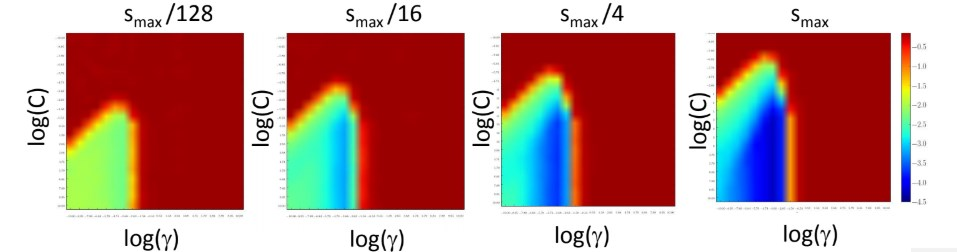
\includegraphics[width=0.9\textwidth]{../w07_hpo_speedup/images/fabolas/example_mnist.jpg}
	    \begin{itemize}
            \item Computational cost grows quadratically in dataset size $z$
            \item Error shrinks smoothly with $z$
        \end{itemize}
	\item Evaluations on the smallest subset (about 400 data points) cost 10\,000$\times$ less than on the full data set
    
\end{itemize}
\end{frame}
%----------------------------------------------------------------------
%----------------------------------------------------------------------

%----------------------------------------------------------------------
%----------------------------------------------------------------------
\begin{frame}[c]{Idea of Multi-fidelity Bayesian optimization \litw{\href{https://dl.acm.org/doi/pdf/10.5555/3305381.3305567}{Kandasamy et al. 2017};  \href{https://arxiv.org/pdf/1605.07079.pdf}{Klein et al. 2016}}}
% https://papers.nips.cc/paper/6118-gaussian-process-bandit-optimisation-with-multi-fidelity-evaluations

\begin{itemize}
	\item Recall: standard Bayesian optimization uses a model $\surro(\conf) \approx y$ to select the next $\conf$
\pause
\medskip
	\item \alert{Multi-fidelity} Bayesian optimization uses a model $\surro(\conf\alert{, z}) \approx y$ to select the next $(\conf\alert{, z})$
	
	\begin{itemize}
		\item Here, $z\in \mathcal{Z}$ is the fidelity; $\mathcal{Z}$ is the fidelity space, e.g., $\mathcal{Z} = [1, N_{\bullet}] \times  [1, T_{\bullet}]$
	\end{itemize}	 
    \pause
    \bigskip
	
%	\item BOCA - a general approach
%	\begin{itemize}
%	    \item Introduces continuity in fidelity space
%		\item Based on \alert{UCB}
%	\end{itemize}
%   
%	\item FABOLAS - a Gaussian process for extrapolating from small to large datasets
%	\begin{itemize}
%		\item This approach uses dataset size as a fidelity $(z \in [0, 1])$
%		\item Based on \alert{Entropy Search}
%	\end{itemize}


    \item Denoting $\alert{z_{\bullet}}$ as the maximum fidelity (e.g., $z_{\bullet} = [N_{\bullet},T_{\bullet}]$), our goal is to find:
        \begin{equation*}
            \optconf = \argmin_{\conf \in \pcs} \func(\conf) = \argmin_{\conf \in \pcs} \surro(\conf, \alert{z_{\bullet}})
        \end{equation*}

    \pause
    \bigskip

    \item Implications for Bayesian optimization
    \begin{itemize}
    	\item Model $\surro$ needs to be good at \alert{extrapolating} from small to large $z$
		\item Acquisition function now also needs to select $z$ (i.e., take into account cost of evaluations)
	\end{itemize}
\end{itemize}




\end{frame}
%----------------------------------------------------------------------
%----------------------------------------------------------------------

%----------------------------------------------------------------------
%----------------------------------------------------------------------
%\begin{frame}[c]{Bayesian Optimization with Continuous Approximations}
%
%\begin{itemize}
%    \item \emph{Goal.} Use the cheap approximations to guide search for the optimum of $\func$, \\ reduce the overall cost of optimization
%    \item \emph{Example.} Tuning of a classification algorithm over a space of hyperparameters $\conf$ 
%        \begin{itemize}
%            \item using $N_{\bullet}$ data points
%            \item via iterative algorithm for $T_{\bullet}$ iterations
%        \end{itemize}
%    \item \emph{Solution.} Approximate validation loss using fewer data points $N < N_{\bullet}$ and/or fewer iterations $T < T_{\bullet}$, such that search deploys:
%        \begin{itemize}
%            \item cheap low fidelity experiments with small $(N, T)$ to discard bad hyperparameters 
%            \item expensive high fidelity experiments with large $(N, T)$ for promising regions
%        \end{itemize}
%    
%\end{itemize}
%\end{frame}
%----------------------------------------------------------------------
%----------------------------------------------------------------------

%----------------------------------------------------------------------
%----------------------------------------------------------------------
%\begin{frame}[c]{Bayesian Optimization with Continuous Approximations}
%
%\begin{itemize}
%
%        \begin{itemize}
%            \item surrogate function $\surro : \alert{\mathcal{Z}} \times \conf \rightarrow  \mathbb{R}$
%            \item e.g. fidelity space $\mathcal{Z} = [1, N_{\bullet}] \times  [1, T_{\bullet}], z_{\bullet} = [N_{\bullet}, T_{\bullet}]$
%
%        \end{itemize}
%
%    \item Determine the fidelity $\iter[\bocount]{z} \in \mathcal{Z}$ to query $\surro$:
%        \begin{enumerate}
%            \item Select a subset  $\iter[\bocount]{Z}$ of $\mathcal{Z}$, that:
%                \begin{itemize}
%                    \item considers only cheaper fidelities,
%                    \item trades of \emph{information gain} and \emph{cost} while enforcing more exploration \\ in cheaper regions in the early stage of the search, %
%                    \item excludes fidelities in a close neighborhood of $z_{\bullet}$.
%                \end{itemize}
%            \item If the subset is empty: $\iter[\bocount]{z} = z_{\bullet}$
%            \item Otherwise: $\iter[\bocount]{z} \in \argmin_{z \in \iter[\bocount]{Z}} \cost(z)$
%        \end{enumerate}
%
%\end{itemize}
%\end{frame}
%----------------------------------------------------------------------
%----------------------------------------------------------------------

% %----------------------------------------------------------------------
% %----------------------------------------------------------------------
% \begin{frame}[c]{Fast Bayesian Optimization on Large Datasets}
% \framesubtitle{Multi-fidelity Bayesian optimization}

% \alert{Multi-fidelity Bayesian optimization} for fidelity with values $z\in \mathcal{Z}$ 
% \begin{itemize}
% 	\item Standard Bayesian optimization uses a model $\func(\conf) \approx y$ to select the next $\conf$
% 	\item \alert{Multi-fidelity Bayesian optimization} uses a model $\func(\conf\alert{, z}) \approx y$ to select the next $(\conf\alert{, z})$
%     \fhpause
%     \smallskip
    
% 	\item Model $\func$ needs to be good at extrapolating from small to large $z$
	
% 	\item E.g., a Gaussian process for extrapolating from small to large datasets - FABOLAS
% 	\begin{itemize}
% 		\item This approach uses dataset size as a fidelity $(z \in [0, 1])$,
% 		\item based on \alert{Entropy Search},
% 		\item achieved 1\,000-fold speedups for SVM on MNIST example.
% 	\end{itemize}
% \end{itemize}
% \end{frame}
% %----------------------------------------------------------------------
% %----------------------------------------------------------------------

%----------------------------------------------------------------------
%----------------------------------------------------------------------
\begin{frame}[c]{Entropy Search: Reminder}

\begin{itemize}
		\item Define the $p_{\text{min}}$ distribution given data $\dataset$:
		$$p_{\text{min}}(\conf^* \mid \alert{\dataset}) := p(\conf^* \in \argmin_{\conf\in \pcs} \func(\conf) \mid \alert{\dataset})$$
	

		\item Entropy search  aims to minimize the entropy \alert{$\mathcal{H}[p_\text{min}]$} \lit{\href{http://jmlr.csail.mit.edu/papers/volume13/hennig12a/hennig12a.pdf}{Hennig and Schuler. 2012}}
		\begin{itemize}
			\item It aims to be maximally certain about the location of $\conf^*$
		\end{itemize}

\bigskip
\pause
		\item In a nutshell: select 
%		\begin{enumerate}
%			\item Estimate $p(\func \mid \dataset)$, e.g., using a GP 
%			\item Approximate $p_\text{min}$ by representer points and Monte-Carlo simulations
%			\item Select 
$\conf$ that maximizes the following acquisition function:
%		\end{enumerate}
\end{itemize}
\vspace*{0.5cm}
	\[{\acq}_{ES}(\conf) := \mathcal{H}[p_{\text{min}}(\cdot \mid \alert{\dataset})] - \mathds{E}_{\alert{p(\tilde{\cost}\mid \conf, \dataset)}} 
	\left[   \mathcal{H}[p_{\text{min}}(\cdot \mid \alert{\dataset \cup \left\langle \conf, \tilde{\cost} \right\rangle })] \right]\]

\end{frame}
%----------------------------------------------------------------------
%----------------------------------------------------------------------

%----------------------------------------------------------------------
%----------------------------------------------------------------------
\begin{frame}[c]{Entropy Search for Multi-Fidelity Optimization \litw{\href{http://proceedings.mlr.press/v54/klein17a/klein17a.pdf}{Klein et al. 2017}}}

\begin{itemize}
		\item We now care about the $p_{\text{min}}$ distribution for the maximal budget $z_{\bullet}$:
		$$p_{\text{min}}(\conf^* \mid \dataset) := p(\conf^* \in \argmin_{\conf\in \pcs} \func(\conf\alert{,z_{\bullet}}) \mid \dataset)$$
	
		\item We still want to minimize the entropy $\mathcal{H}[p_\text{min}]$
\pause
\medskip
		\item Now we aim for the biggest \alert{reduction in entropy per time spent}
		\begin{itemize}
			\item Now we don't model only $\func$, but also \alert{the cost $c(\conf,z)$}
			\item We choose the next $(\conf,z)$ by maximizing:
		\end{itemize}
\end{itemize}
\vspace*{0.5cm}
	\[{\acq}_{ES}(\conf,z \mid \dataset) := \mathds{E}_{\alert{p(\tilde{\cost}\mid (\conf, z), \dataset)}} 
	\left[   \frac{\mathcal{H}[p_{\text{min}}(\cdot \mid \alert{\dataset})] - \mathcal{H}[p_{\text{min}}(\cdot \mid \alert{\dataset \cup \left\langle (\conf,z), \tilde{\cost} \right\rangle}}{\alert{c(\conf,z)}} \right]\]

%	\item Introduced to handle large datasets, in paper ``Fast Bayesian Optimization on Large Datasets (Fabolas)'' by \lit{\href{http://proceedings.mlr.press/v54/klein17a/klein17a.pdf}{Klein, Falkner \& Hutter, 2017}}

\end{frame}
%----------------------------------------------------------------------
%----------------------------------------------------------------------

%----------------------------------------------------------------------
%----------------------------------------------------------------------
\begin{frame}[c]{Entropy Search for Multi-Fidelity Optimization \litw{\href{http://proceedings.mlr.press/v54/klein17a/klein17a.pdf}{Klein et al. 2017}}}

\begin{itemize}
    \item The entire algorithm iterates the following 2 steps until time is up:
		\begin{enumerate}
			\item Select $(\conf,z)$ by maximizing:
    			\[{\acq}_{ES}(\conf,z \mid \dataset) := \mathds{E}_{\alert{p(\tilde{\cost}\mid (\conf, z), \dataset)}} 
            	\left[   \frac{\mathcal{H}[p_{\text{min}}(\cdot \mid \alert{\dataset})] - \mathcal{H}[p_{\text{min}}(\cdot \mid \alert{\dataset \cup \left\langle (\conf,z), \tilde{\cost} \right\rangle}}{\alert{c(\conf,z)}} \right]\]
			\item Observe performance $f(\conf,z)$ and cost $c(\conf,z)$ and update models for $f$ and $c$ 
		\end{enumerate}

\pause

    \item The algorithm originally focussed on data subsets and is therefore dubbed \\ \alert{Fabolas}: 
    ``Fast Bayesian Optimization on Large Datasets''
	
\pause

\begin{columns}[T] % align columns
\begin{column}{.48\textwidth}


    \begin{block}{Advantages}
    \begin{itemize}
    	\item Conceptually beautiful
    	\item 1\,000-fold speedups for optimizing SVMs on MNIST
    \end{itemize}
    \end{block}
\pause
\end{column}%

\hfill%

\begin{column}{.48\textwidth}

    \begin{block}{Disadvantages}
    \begin{itemize}
    	\item \alert{Scalability} of GPs is a big problem (limits size of initial design)
    	\item Limited applicability of Gaussian processes
    \end{itemize}
\end{block}

\end{column}
\end{columns}   

\end{itemize}
\end{frame}
%----------------------------------------------------------------------
%----------------------------------------------------------------------


% %----------------------------------------------------------------------
% %----------------------------------------------------------------------
% \begin{frame}[c]{Fast Bayesian Optimization on Large Datasets}
% \framesubtitle{Overview}

% \begin{itemize}
%     \item Automatically choose dataset size for each evaluation
%         \begin{itemize}
%             \item Include extra dimension in probabilistic model to capture \\ dependence on dataset size $s$: $\func(\conf, s)$
%             \item Construct a second model for computational cost: $\cost(\conf, s)$
%             \item Trade off information gain about global optimum vs. cost
%         \end{itemize}
%     \item Extend the GP by an additional input dimension: $s \in [0, 1]$
%         \begin{itemize}
%             \item standard stationary kernel (over HPs) + covariance function in $s$
%                 \begin{equation*}
%                     \kernel( (\conf, s), (\conf', s') ) = \kernel_{5/2} (\conf, \conf') ( \phi^{T}(s) * \Sigma_{\phi} * \phi(s') )
%                 \end{equation*}
%             \item  we use the same form of kernel to model the loss $\func$ and cost $\cost$, but with different basis functions $\phi_{\func}$ and $\phi_{\cost}$
%                 \begin{itemize}
%                     \item $\phi_{\func}(s) = (1, (1-s)^2)^T$
%                     \item $\phi_{\cost}(s) = (1, s)^T$
%                 \end{itemize}
%         \end{itemize}
        
% \end{itemize}

% \source{Klein, Bartels, Falkner, Hennig, Hutter, AISTATS 2017}
% \end{frame}
% %----------------------------------------------------------------------
% %----------------------------------------------------------------------

%----------------------------------------------------------------------


\begin{frame}{Questions to Answer for Yourself / Discuss with Friends}

\bigskip

\begin{itemize}
    \item \alert{Discussion.} What kind of cost model would you use in Fabolas?
\medskip
	\item \alert{Discussion.} Could one use an acquisition function other than entropy search for Fabolas?    

\end{itemize}

\end{frame}
\end{document}